% !TeX spellcheck = en_GB

~
\pagebreak

\section{Challenges}\label{Challenges}
While building the generic version of Hibernate Search, we will encounter some challenges. First, we will introduce a small example project. We will then use this project to illustrate the biggest challenges. It will also be used to showcase some problems and usages later on in this thesis.

\subsection{The example project} \label{example_project}
Consider a software built with JPA that is used to manage the inventory of a bookstore. It stores information about the available books (ISBN, title, genre, short summary of the contents) and the corresponding authors (surrogate id, first \& last name, country) in a relational database. Each author is related to zero or more Books and each Book is written by one or more Authors. The entity relationship model diagram defining the database looks like this:
\\
\begin{figure}[ht]
	\centering
	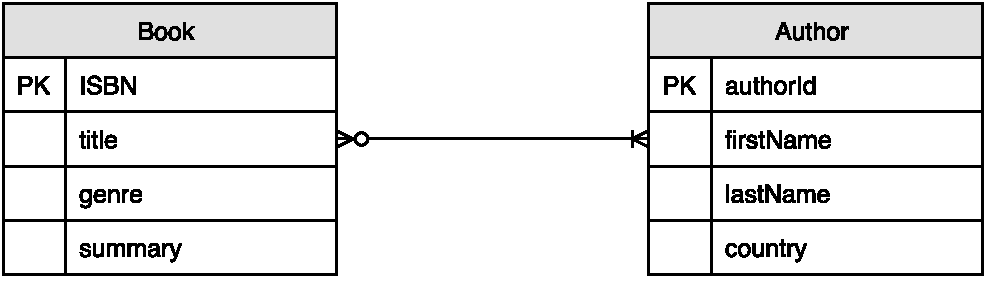
\includegraphics[scale = 0.9]{images/Sample_Project_ER.pdf}
	\caption{the bookstore entity relationship model}
	\label{fig3}
\end{figure}
\\
Using a mapping table for the M:N relationship of Author and Book, the database contains three tables: Author, Book and Author\_Book. The applications strictly uses JPA to access the data without any vendor specific features. The JPA annotated classes for these entities are defined as shown in the following listings.

\pagebreak

\lstset{language=java}
\begin{lstlisting}[frame=htrbl, caption={Book.java}, label={lst:book.java_1}]
@Entity
@Table(name = "Book")
public class Book {

	@Id
	@Column(name = "isbn")
	private String isbn;
	
	@Column(name = "title")
	private String title;
	
	@Column(name = "genre")
	private String genre;
	
	@Lob
	@Column(name = "summary")
	private String summary;
	
	@ManyToMany(mappedBy = "books", cascade = {
		CascadeType.MERGE,
		CascadeType.DETACH,
		CascadeType.PERSIST,
		CascadeType.REFRESH
	})
	private Set<Author> authors;
	
	//getters & setters ...
}
\end{lstlisting}

\pagebreak

\lstset{language=java}
\begin{lstlisting}[frame=htrbl, caption={Author.java}, label={lst:author.java_1}]
@Entity
@Table(name = "Author")
public class Author {
	
	@Id
	@GeneratedValue(strategy = GenerationType.AUTO)
	@Column(name = "authorId")
	private Long authorId;
	
	@Column(name = "firstName")
	private String firstName;
	
	@Column(name = "lastName")
	private String lastName;
	
	@Column(name = "country")
	private String country;
	
	@ManyToMany(cascade = {
		CascadeType.MERGE, 
		CascadeType.DETACH, 
		CascadeType.PERSIST, 
		CascadeType.REFRESH
	})
	@JoinTable(name = "Author_Book", 
		joinColumns = 
			@JoinColumn(name = "authorFk", 
				referencedColumnName = "authorId"),
		inverseJoinColumns = 
			@JoinColumn(name = "bookFk", 
				referencedColumnName = "isbn"))
	private Set<Book> books;
	
	//getters & setters ...
}
\end{lstlisting}
For the sake of simplicity and since every JPA provider is able to derive a default DDL script from the annotations, we don't supply any information about how to create the database schema here. However, for real world applications defining a hand-written DDL script might be a better idea since the generated code might not be optimal and could differ between the different JPA implementations and RDBMSs used.

\pagebreak

\subsection{Standalone version} \label{problem_indexing_searching}
Hibernate Search's engine wasn't designed to be used directly by application developers. Its main purpose is to serve as an integration point for other APIs that need to leverage its power to index object graphs and query the index for hits by exposing a quite low-level and in some ways complex API. This is why we have to write our own standalone version based on the "hibernate-search-engine" serving as an abstraction layer such that it eases the usage of the engine in our JPA integration.

\subsection{JPA integration}
After the standalone version is finished, we will build an integration of it with JPA. By incorporating the same engine that the original does, we will support the same indexing behaviour and even stay compatible with entities designed for the original with as little changes as possible. In fact, the main goal for the JPA integration is to be as compatible as possible with Hibernate Search ORM.
\\\\\
The implementations of these two challenges are represented by the modules "Hibernate Search Standalone" and "Hibernate Search GenericJPA" in the following figure \ref{hibernate_search_genericjpa_complete_architecture}. Together with the module "Hibernate Search Database Utilities", these are the submodules of our complete generic version and the result of the top-bottom analysis as described in chapter \ref{Methods}. Note that during this thesis we will be referring to the whole project by the name of the main module "Hibernate Search GenericJPA" as well.

\begin{figure}[ht]
	\centering
	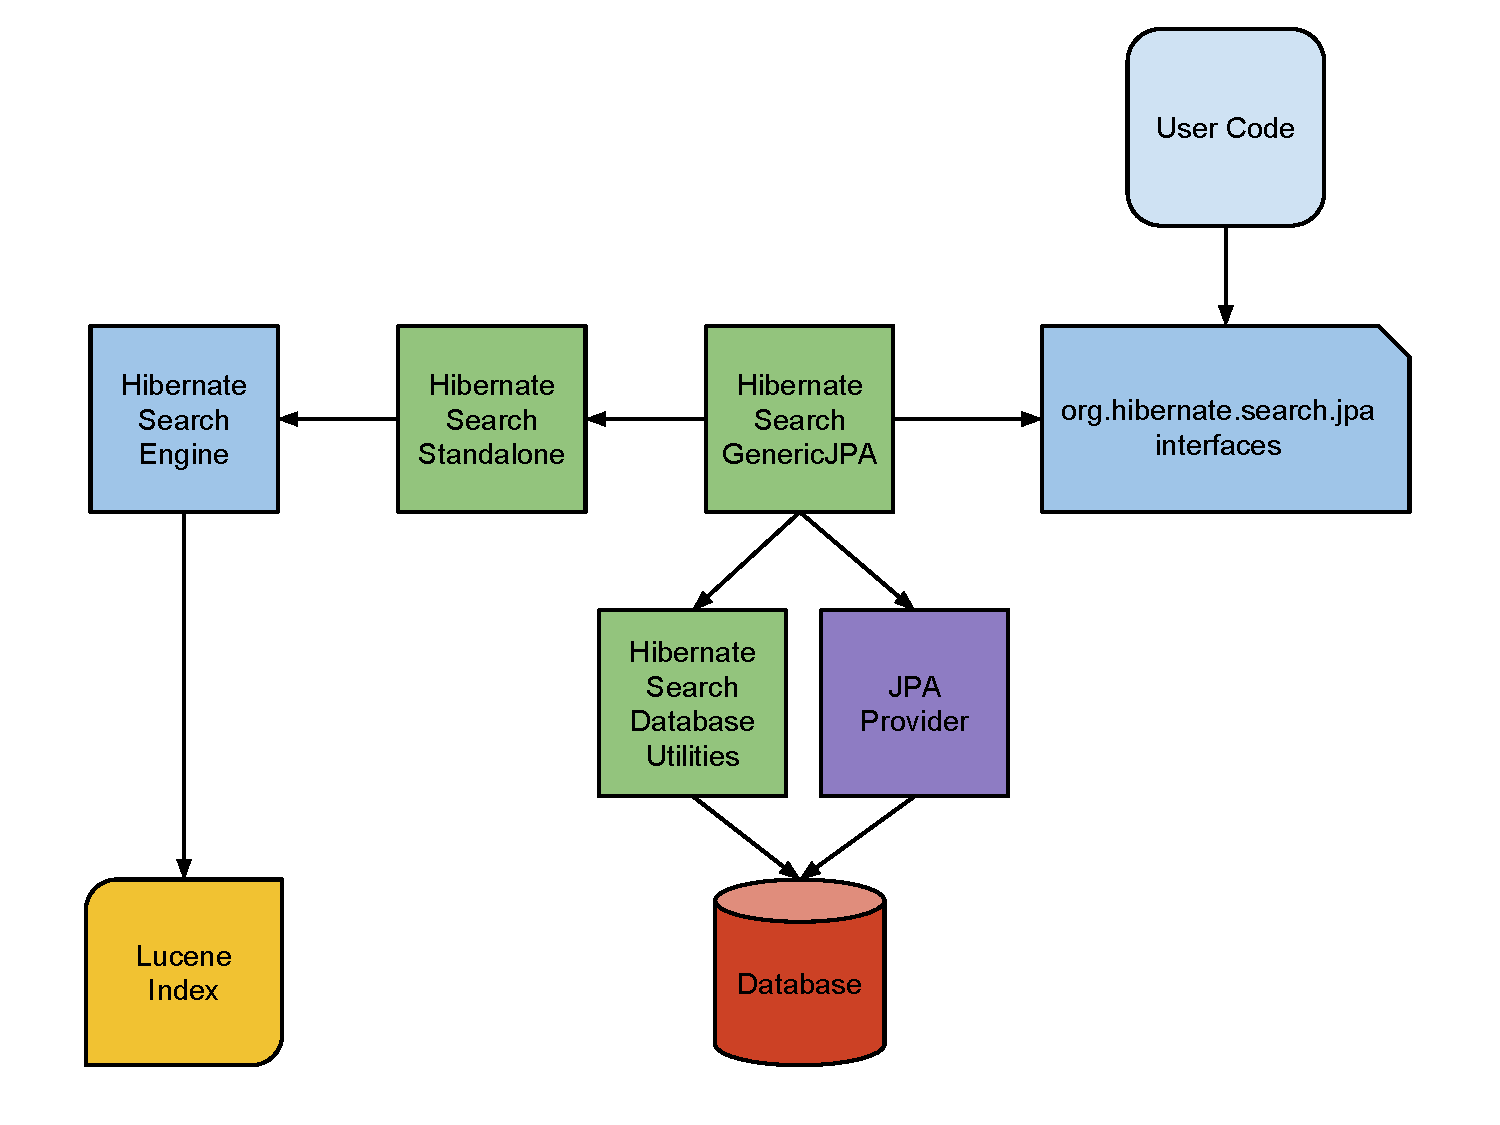
\includegraphics[scale=0.5]{images/hibernate_search_genericjpa_complete_architecture.pdf}
	\caption{Complete Architecture of Hibernate Search GenericJPA}
	\label{hibernate_search_genericjpa_complete_architecture}
\end{figure}

\pagebreak

%\subsection{Index rebuilding}
%If the way objects are indexed changes, the existing files have to %be purged and recreated in the new index format. The naive approach %here would be purging the index and then indexing all data %sequentially as they are retrieved from the database:
%\\
%\lstset{language=java}
%\begin{lstlisting}[frame=htrbl, caption={naive index rebuilding}, %label={lst:naiveIndexing}]
%EntityManager em = ...;
%<Hibernate Search Controller> search = ...;
%
%search.purgeAll(Book.class);
%
%Query query = em.createQuery("SELECT b FROM Book b");
%List<Book> booksFromDb = query.getResultList();
%for(Book b : booksFromDb) {
%	search.index(b);
%}
%\end{lstlisting}
%While this might work for small databases, bigger datasets will %cause this algorithm to run out of memory, since we just retrieve %all the data at once. This could be fixed by implementing a %batching strategy, but it would still be quite slow as it only uses %one thread which would mostly be used for I/O from the database.
%\\\\
%This is not optimal, since a index rebuild should be as fast as %possible as the application cannot be properly used while the job %is running. Therefore we need to create a parallel indexing %mechanism, just like the one Hibernate Search ORM has.

\subsection{Automatic index updating} \label{automatic_indexing_problematic_intro}
The most important feature to be re-built, is automatic index updating. In Hibernate Search ORM, every change in the database is automatically reflected in the index. It is important to have this feature, because otherwise developers would have to manually make sure the index is always up-to-date. With bigger project sizes it gets increasingly harder to keep track of all the locations in the code that change index relevant data and inconsistencies in the indexing logic become nearly unavoidable. While this problem might be mitigated by hiding all the database access logic behind a service layer, even such a solution would be hard to keep error-free as for big applications this layer will probably have multiple critical indexing relevant spots as well.
\\\\
The original Hibernate Search ORM is achieving an up-to-date index by listening to specific Hibernate ORM events for all of the C\_UD (CREATE, UPDATE, DELETE) actions. These events also cover entity relationship collections (for example represented by mapping tables like Author\_Book). As our goal is to create a generic Hibernate Search engine that works with any JPA implementation, we cannot rely on any vendor specific event system. Thus, at least an additional generic solution has to be found.
\\\\
This feature will be part of the "Hibernate Search GenericJPA" module.

\subsection{Timeline}
The solutions for the challenges depend on each other in the same order they were described above: the JPA integration can only be worked on as soon as the standalone integration is done and work on the automatic updating mechanism cannot be started without knowing the JPA integration interfaces. The timeline of our project therefore looks like this:
\\
\begin{figure}[ht]
	\centering
	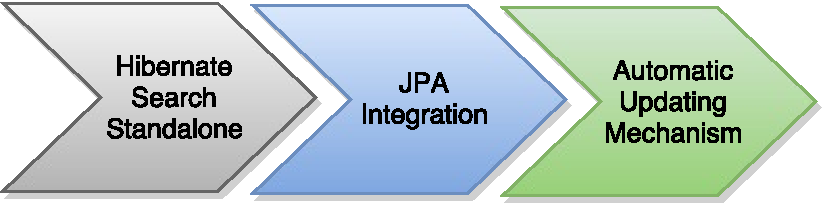
\includegraphics[scale=0.75]{images/timeline_genericjpa_complete.pdf}
	\caption{Timeline of the project}
	\label{project_timeline}
\end{figure}

\pagebreak